\documentclass{article}
\usepackage{tikz}
\usetikzlibrary{arrows.meta, positioning, shapes.geometric}
\usepackage[utf8]{inputenc}
\usepackage[most]{tcolorbox} % 在前言區加入
\usepackage[UTF8]{ctex}
\usepackage{pgfplots}
\pgfplotsset{compat=1.16}
\usetikzlibrary{calc}
\usepackage{amsmath}
\usepackage[siunitx]{circuitikz}
\usepackage{xcolor}
\usepackage{amssymb}
\usepackage{array}
\usepackage{booktabs}
\usepackage{physics}
\usepackage{siunitx}
\usepackage{enumitem}
\usepackage{subcaption}
\usepackage{pgfplots}
\pgfplotsset{compat=1.16}
\pgfmathdeclarefunction{Jzero}{1}{%
  \pgfmathparse{
    ( (#1) <= 8 ) ?
      ( 1 - ( (#1)^2 )/4 + ( (#1)^4 )/64
        - ( (#1)^6 )/2304 + ( (#1)^8 )/147456
        - ( (#1)^10 )/14745600 )
      :
      ( sqrt(2/(pi*(#1))) * cos(deg( (#1) - pi/4 )) )
  }%
}
\usepackage[unicode]{hyperref}
\pdfstringdefDisableCommands{%
  \def\pi{pi}%
  \def\Omega{Omega}%
  \def\hat#1{#1}%
  \def\dfrac#1#2{#1/#2}%
  \def\int{\text{∫}}%
}
\usepackage{xeCJK}
\usepackage{bm}
\usepackage{CJKutf8}
\setCJKmainfont{Noto Serif CJK TC}    % 思源宋體繁體版(推薦)
\setCJKsansfont{Microsoft JhengHei}   % 微軟正黑體
\setCJKmonofont{Noto Sans Mono CJK TC}

\begin{document}
\noindent
In a general nonlinear state-space system
\[
\dot{x} = f(t, x, u), \qquad y = h(t, x, u),
\]
an \emph{equilibrium point} $(x_e, u_e)$ is a state–input pair such that, if the system starts there, it remains there forever.  
That is,
\[
\dot{x} = 0 \quad \text{when } x = x_e,\, u = u_e,
\]
or equivalently,
\[
f(t, x_e, u_e) = 0.
\]
The corresponding output at equilibrium is
\[
y_e = h(t, x_e, u_e).
\]

\bigskip
\noindent
\textbf{Isolated vs.\ continuum of equilibrium points.}
\begin{itemize}
  \item \textbf{Isolated equilibrium:} There is only one equilibrium point in its neighborhood.  
  Example:
  \[
  \dot{x} = -x,
  \]
  which has a single equilibrium at $x=0$.
  
  \item \textbf{Continuum of equilibria:} There exists an infinite (continuous) set of equilibrium points forming a line, plane, or manifold.  
  Example:
  \[
  \dot{x}_1 = 0, \qquad \dot{x}_2 = -x_2,
  \]
  where any state of the form $(x_1, 0)$ is an equilibrium.  
  This is called a \emph{continuum of equilibrium points} (平衡點連續).
\end{itemize}

\bigskip
\noindent
\textbf{Linear systems.}
For a linear time-varying system,
\[
\dot{x} = A(t)x + B(t)u, \qquad y = C(t)x + D(t)u,
\]
which is a special case of the nonlinear model above where $f$ and $h$ are linear in $x$ and $u$.

\bigskip
\noindent
\textbf{Equilibria in linear systems.}
For the time-invariant case,
\[
0 = A x_e + B u_e.
\]
\begin{itemize}
  \item If $A$ is invertible, there is a single (isolated) equilibrium:
  \[
  x_e = -A^{-1} B u_e.
  \]
  \item If $A$ is singular, there exists a \emph{continuum of equilibria.}
\end{itemize}
\noindent
\textbf{Multiple isolated equilibria.}
A linear system can have only one isolated equilibrium point; thus, it has only one steady-state operating point that attracts all trajectories (if stable).

\bigskip
\noindent
For a nonlinear system,
\[
\dot{x} = f(x, u),
\]
there may exist more than one isolated equilibrium point, i.e.\ multiple distinct solutions of
\[
f(x_e, u_e) = 0.
\]
The state of the system may converge to one of several steady-state operating points,
depending on the \emph{initial state of the system}.
Each equilibrium has its own \emph{basin of attraction}.
\noindent
\textbf{多個孤立平衡點(Multiple isolated equilibria)} \\[4pt]
對於\textbf{線性系統}而言,
它只能有一個孤立的平衡點,因此也只有一個穩態工作點(steady-state operating point)。
若系統是穩定的,所有狀態最終都會收斂到該唯一的平衡點,與初始狀態無關。

\bigskip
\noindent
對於\textbf{非線性系統}
\[
\dot{x} = f(x, u),
\]
可能存在多組滿足
\[
f(x_e, u_e) = 0
\]
的解 $(x_e, u_e)$,也就是\textbf{多個孤立平衡點}。

\bigskip
\noindent
系統的狀態可能會根據\textbf{初始狀態}不同,
而收斂到不同的平衡點。  
每個平衡點附近的區域稱為其\textbf{吸引域(basin of attraction)}。

\bigskip
\noindent
\textbf{舉例:}
\[
\dot{x} = x - x^3
\]
滿足平衡條件 $0 = x - x^3$,得到三個孤立平衡點:
\[
x_e = 0, \ \pm 1.
\]
此系統中,初始狀態決定了最終收斂到哪一個平衡點。
% Compile with: \usepackage{pgfplots}  (and \pgfplotsset{compat=newest})
\begin{center}
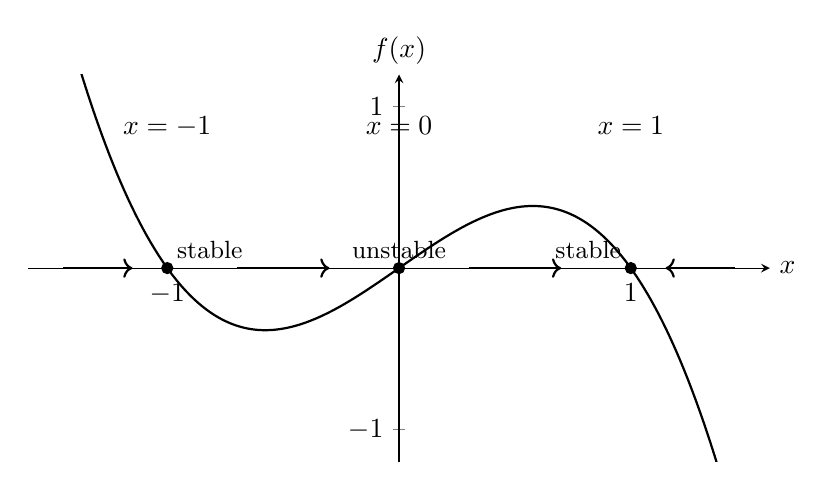
\begin{tikzpicture}
  \begin{axis}[
    width=11cm, height=6.5cm,
    axis lines=middle,
    xmin=-1.6, xmax=1.6,
    ymin=-1.2, ymax=1.2,
    xlabel={$x$}, ylabel={$f(x)$},
    xtick={-1,0,1}, ytick={-1,0,1},
    domain=-1.6:1.6, samples=201,
    enlargelimits=false,
    every axis x label/.style={at={(current axis.right of origin)}, anchor=west},
    every axis y label/.style={at={(current axis.above origin)}, anchor=south}
  ]

    % The function f(x) = x - x^3
    \addplot[thick] {x - x^3};

    % Equilibria (real roots)
    \addplot[only marks, mark=*, mark size=2pt] coordinates {(-1,0) (0,0) (1,0)};

    % Labels for equilibria
    \node[below] at (axis cs:-1,1) {$x=-1$};
    \node[below] at (axis cs:0,1) {$x=0$};
    \node[below] at (axis cs:1,1) {$x=1$};

    % Flow arrows on x-axis (showing sign of \dot{x} = f(x))
    \draw[->, thick] (axis cs:-1.45,0) -- (axis cs:-1.15,0); % x<-1 : right
    \draw[->, thick] (axis cs:-0.7,0) -- (axis cs:-0.3,0);   % -1<x<0 : left (reverse arrow)
    \draw[->, thick] (axis cs:0.3,0) -- (axis cs:0.7,0);     % 0<x<1 : right
    \draw[->, thick] (axis cs:1.45,0) -- (axis cs:1.15,0);   % x>1 : left

    % Stability hints
    \node[above right] at (axis cs:-1,0) {\small stable};
    \node[above]       at (axis cs:0,0)  {\small unstable};
    \node[above left]  at (axis cs:1,0)  {\small stable};

  \end{axis}
\end{tikzpicture}
\end{center}
\noindent
\textbf{不穩定平衡(Unstable Equilibrium)}

\bigskip
\noindent
考慮一個一維自主系統:
\[
\dot{x} = f(x).
\]
若存在某一點 $x = x_e$ 使得
\[
f(x_e) = 0,
\]
則 $x_e$ 為系統的\textbf{平衡點(equilibrium point)}。  
當系統狀態位於該點時,$\dot{x}=0$,狀態將保持不變。

\bigskip
\noindent
\textbf{穩定與不穩定的差異如下:}

\begin{center}
\begin{tabular}{|c|c|c|c|}
\hline
\textbf{類型} & \textbf{微小擾動後的行為} & \textbf{幾何意義} & \textbf{物理比喻} \\
\hline
穩定平衡 (Stable) & 狀態回到原平衡點 & 周圍箭頭指向該點 & 小球在碗底 \\
\hline
不穩定平衡 (Unstable) & 狀態遠離原平衡點 & 周圍箭頭遠離該點 & 小球在山頂 \\
\hline
\end{tabular}
\end{center}

\bigskip
\noindent
\textbf{數學上(Lyapunov 意義)}:

若對任意 $\varepsilon > 0$,存在 $\delta > 0$,使得當 $|x(0) - x_e| < \delta$ 時,  
系統軌跡滿足 $|x(t) - x_e| < \varepsilon$ 對所有 $t > 0$ 皆成立,則稱 $x_e$ \textbf{穩定}。  
反之,若存在再小的擾動都會使軌跡離開該點附近,則 $x_e$ 為\textbf{不穩定平衡點}。

\bigskip
\noindent
\textbf{範例:}
\[
\dot{x} = x - x^3
\]
其平衡條件為:
\[
x - x^3 = 0 \quad \Rightarrow \quad x_e = -1, 0, 1.
\]

取導數:
\[
f'(x) = 1 - 3x^2.
\]
代入:
\[
f'(-1) = -2 < 0 \Rightarrow \text{穩定}, \qquad
f'(0) = 1 > 0 \Rightarrow \text{不穩定}, \qquad
f'(1) = -2 < 0 \Rightarrow \text{穩定}.
\]

因此,$x=0$ 為\textbf{不穩定平衡點},
而 $x=\pm1$ 為\textbf{穩定平衡點}。

\bigskip
\noindent
\textbf{圖像化理解:}
\[
\text{當 } f(x)>0 \Rightarrow \dot{x}>0 \text{(狀態向右移動)}, \quad
f(x)<0 \Rightarrow \dot{x}<0 \text{(狀態向左移動)}.
\]
若在平衡點兩側,箭頭「遠離」該點,則該點為\textbf{不穩定平衡}。

\begin{center}
\begin{figure}[h!]
  \centering
  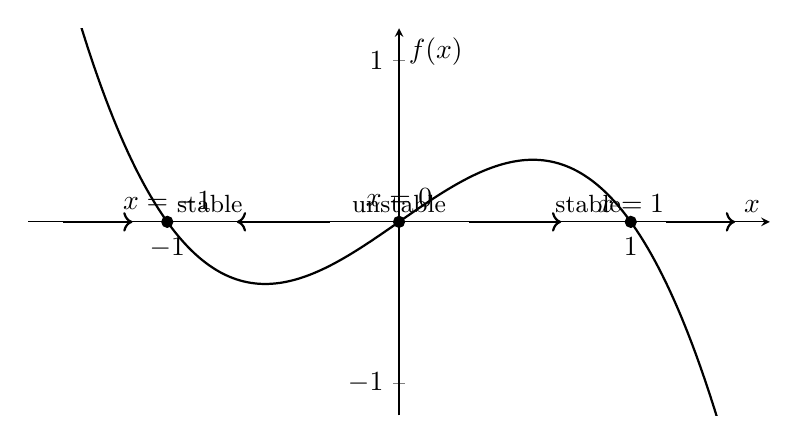
\begin{tikzpicture}
    \begin{axis}[
      width=11cm, height=6.5cm,
      axis lines=middle,
      xmin=-1.6, xmax=1.6,
      ymin=-1.2, ymax=1.2,
      xlabel={$x$}, ylabel={$f(x)$},
      xtick={-1,0,1}, ytick={-1,0,1},
      domain=-1.6:1.6, samples=201
    ]
      % Plot f(x)
      \addplot[thick] {x - x^3};

      % Mark equilibria
      \addplot[only marks, mark=*, mark size=2pt] coordinates {(-1,0) (0,0) (1,0)};
      \node[above] at (axis cs:-1,0) {$x=-1$};
      \node[above, yshift=2pt] at (axis cs:0,0) {$x=0$};
      \node[above] at (axis cs:1,0) {$x=1$};

      % Flow arrows
      \draw[->, thick] (axis cs:-1.45,0) -- (axis cs:-1.15,0);
      \draw[<-, thick] (axis cs:-0.7,0) -- (axis cs:-0.3,0);
      \draw[->, thick] (axis cs:0.3,0) -- (axis cs:0.7,0);
      \draw[<-, thick] (axis cs:1.45,0) -- (axis cs:1.15,0);

      % Stability labels
      \node[above right] at (axis cs:-1,0) {\small stable};
      \node[above] at (axis cs:0,0) {\small unstable};
      \node[above left] at (axis cs:1,0) {\small stable};
    \end{axis}
  \end{tikzpicture}
  \caption{相圖示意:$f(x)=x-x^3$,其中 $x=0$ 為不穩定平衡,$x=\pm1$ 為穩定平衡。}
\end{figure}
\end{center}
\section*{Tunnel Diode}

A \textbf{tunnel diode} (also called an \textit{Esaki diode}) is a special type of semiconductor diode that exhibits \textbf{negative resistance} due to the phenomenon of \textbf{quantum tunneling} inside its p--n junction.

\subsection*{1. Construction}

A tunnel diode is fabricated similarly to a normal p--n junction diode, but with \textbf{extremely heavy doping} on both sides --- about \( 10^3 \) times higher than that of an ordinary diode.

Because of the very high doping concentration:
\begin{itemize}
    \item The \textbf{depletion layer} becomes extremely narrow (a few nanometers).
    \item Electrons can \textbf{tunnel} through the potential barrier even when they do not have enough classical energy to overcome it.
\end{itemize}

This tunneling mechanism gives rise to a unique current--voltage characteristic.

\subsection*{2. Current--Voltage Characteristic}

The \( i\text{--}v \) curve of a tunnel diode has three distinct regions:

\[
\begin{array}{c|c|l}
\text{Region} & \text{Voltage range} & \text{Behavior / Description} \\ \hline
1. \text{Tunneling region} & \text{Small forward bias} & \text{Current rises rapidly due to tunneling.} \\
2. \text{Negative resistance region} & \text{Medium bias} & \text{Current decreases as voltage increases.} \\
3. \text{Forward conduction region} & \text{High bias} & \text{Current rises again (normal diode behavior).}
\end{array}
\]

Graphically, it appears as an ``N'' or ``S'' shaped curve:

\[
\frac{di}{dv} < 0 \quad \text{in the negative resistance region.}
\]

\subsection*{3. Negative Resistance}

In the middle region, as the voltage \( v \) increases, the current \( i \) actually decreases, giving
\[
\frac{di}{dv} < 0
\]
This property is known as \textbf{negative differential resistance}, which allows the tunnel diode to:
\begin{itemize}
    \item Amplify small signals,
    \item Generate oscillations,
    \item Operate at extremely high switching speeds.
\end{itemize}

\subsection*{4. Typical Parameters}

\[
\begin{array}{lcl}
V_p & : & \text{Peak voltage (typically } 0.1\text{--}0.3~\text{V)} \\
I_p & : & \text{Peak current (a few mA)} \\
V_v & : & \text{Valley voltage (}0.3\text{--}0.6~\text{V)} \\
I_v & : & \text{Valley current, smaller than } I_p
\end{array}
\]

\subsection*{5. Applications}

Thanks to its negative resistance and high-speed behavior, tunnel diodes are widely used in:
\begin{itemize}
    \item High-frequency oscillators,
    \item Microwave amplifiers,
    \item Fast-switching circuits,
    \item Bistable multivibrators (memory elements).
\end{itemize}

\subsection*{6. Historical Note}

The tunnel diode was invented by \textbf{Leo Esaki} in 1957.  
He was awarded the \textbf{Nobel Prize in Physics} in 1973 for discovering the tunneling phenomenon in semiconductors.

\bigskip
\noindent
\textbf{Summary:}
\[
\boxed{
\text{A tunnel diode is a heavily doped p--n junction device that exhibits negative resistance due to quantum tunneling.}
}
\]
\begin{figure}[htbp]

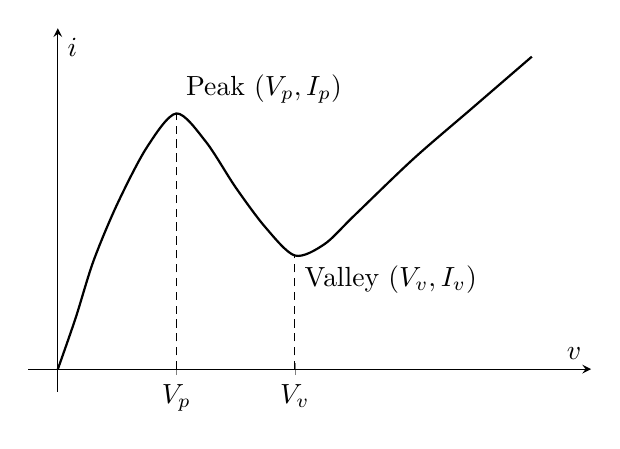
\begin{tikzpicture}
\begin{axis}[
  width=0.72\linewidth, height=6.2cm,
  axis lines=middle, xlabel={$v$}, ylabel={$i$},
  xmin=-0.05, xmax=0.90, ymin=-0.2, ymax=3.0,
  xtick={0,0.2,0.4}, xticklabels={$0$,$V_p$,$V_v$},
  ytick=\empty, domain=0:0.9, samples=200,
  enlargelimits=false, clip=false
]
  % Tunnel-diode I–V (stylized): rise → negative resistance → rise
  \addplot[thick, smooth]
    coordinates {
      (0.00,0.00) (0.03,0.45) (0.06,0.95) (0.10,1.45)
      (0.15,1.95) (0.20,2.25) % peak near Vp
      (0.25,2.00) (0.30,1.60) (0.35,1.25) (0.40,1.00) % valley near Vv
      (0.45,1.10) (0.50,1.35) (0.60,1.85) (0.70,2.30) (0.80,2.75)
    };

  % Vertical guides at Vp and Vv
  \addplot[densely dashed] coordinates {(0.20,0) (0.20,2.25)};
  \addplot[densely dashed] coordinates {(0.40,0) (0.40,1.00)};

  % Labels for peak and valley
  \node[anchor=south west] at (axis cs:0.20,2.25) {Peak $(V_p,I_p)$};
  \node[anchor=north west] at (axis cs:0.40,1.00) {Valley $(V_v,I_v)$};
\end{axis}
\end{tikzpicture}
\caption{Tunnel diode \(i\text{--}v\) characteristic showing the negative-resistance region between \(V_p\) and \(V_v\).}
\end{figure}
\section*{Symmetric Tunnel-Diode Characteristic}

Consider a circuit consisting of two \textbf{tunnel diodes} connected in opposite directions, 
each in series with a \SI{0.3}{V} bias source:

\[
\text{Positive branch: } \; \text{Diode conducts for } v > +0.3~\text{V}, \quad
\text{Negative branch: } \; \text{Diode conducts for } v < -0.3~\text{V}.
\]

Because of the opposite orientations, the overall element exhibits a 
\textbf{symmetric nonlinear current--voltage characteristic} described by
\[
i = h(v), \qquad \text{with } h(-v) = -h(v).
\]

\subsection*{1. Right-hand side of the curve (\(v > 0\))}
When the applied voltage \(v\) exceeds approximately \(+0.3~\text{V}\):
\begin{itemize}
    \item The tunnel diode oriented for forward conduction becomes active.
    \item The current \(i\) first increases rapidly (tunneling region), 
          then decreases (negative-resistance region),
          and finally rises again (normal forward conduction).
\end{itemize}
This produces the \textbf{right-hand lobe} of the \(i\!-\!v\) curve.

\subsection*{2. Left-hand side of the curve (\(v < 0\))}
When \(v\) becomes less than approximately \(-0.3~\text{V}\):
\begin{itemize}
    \item The oppositely oriented tunnel diode is forward biased.
    \item It exhibits the same behavior as the first diode but with reversed polarity.
\end{itemize}
Thus, the left-hand side of the curve is the \textbf{mirror image} of the right-hand side.

\subsection*{3. Around \(v = 0\)}
For small voltages \(|v| < 0.3~\text{V}\), both diodes are reverse biased,
and the current is negligible (\(i \approx 0\)).
The overall curve passes smoothly through the origin.

\subsection*{4. Combined characteristic}
The complete \(i = h(v)\) characteristic is shown below.

\begin{figure}[htbp]
\centering
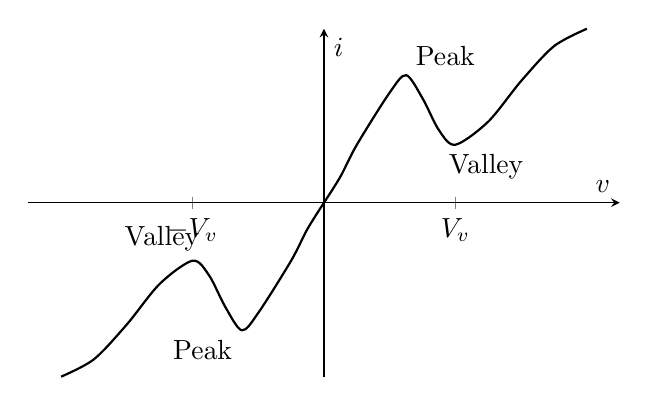
\begin{tikzpicture}
\begin{axis}[
    width=0.75\linewidth, height=6cm,
    axis lines=middle,
    xlabel={$v$}, ylabel={$i$},
    xmin=-0.9, xmax=0.9, ymin=-3, ymax=3,
    xtick={-0.4,0,0.4}, xticklabels={$-V_v$,$0$,$V_v$},
    ytick=\empty,
    domain=-0.8:0.8, samples=200,
    enlargelimits=false, clip=false,
]
    % Right half (positive voltage diode)
    \addplot[thick, smooth, domain=0:0.8]
      coordinates {
        (0.00,0.00) (0.05,0.45) (0.10,1.00) (0.20,1.90)
        (0.25,2.20) (0.30,1.80) (0.35,1.25) (0.40,1.00)
        (0.50,1.40) (0.60,2.10) (0.70,2.70) (0.80,3.00)
      };
    % Left half (mirror)
    \addplot[thick, smooth, domain=-0.8:0]
      coordinates {
        (-0.80,-3.00) (-0.70,-2.70) (-0.60,-2.10) (-0.50,-1.40)
        (-0.40,-1.00) (-0.35,-1.25) (-0.30,-1.80) (-0.25,-2.20)
        (-0.20,-1.90) (-0.10,-1.00) (-0.05,-0.45) (0.00,0.00)
      };
    % Labels
    \node[anchor=south west] at (axis cs:0.25,2.2) {Peak};
    \node[anchor=north west] at (axis cs:0.35,1.0) {Valley};
    \node[anchor=north east] at (axis cs:-0.25,-2.2) {Peak};
    \node[anchor=south east] at (axis cs:-0.35,-1.0) {Valley};
\end{axis}
\end{tikzpicture}
\caption{Symmetric tunnel-diode characteristic \(i = h(v)\) produced by two oppositely oriented tunnel diodes.}
\end{figure}

\bigskip
\noindent
\textbf{Summary:} \\
Each half of the curve corresponds to one tunnel diode's forward-bias behavior.  
The right side arises from the diode conducting for positive voltages,  
while the left side is its mirror image for negative voltages.  
Together they form a symmetric nonlinear element with regions of 
\textbf{negative differential resistance}.
\begin{circuitikz}
  % --- optional yellow background ---
  \fill[yellow!55] (-0.7,-0.8) rectangle (6.2,2.8);

  % Nodes
  \coordinate (LT) at (0,2);   % left, top terminal
  \coordinate (LB) at (0,0);   % left, bottom terminal
  \coordinate (RT) at (6,2);   % right, top corner
  \coordinate (RB) at (6,0);   % right, bottom corner
  \coordinate (XL) at (2,2);   % left vertical branch (top)
  \coordinate (XR) at (4,2);   % right vertical branch (top)

  % Top and bottom buses with open terminals on the left
  \draw (LT) to[short, o-] (XL) -- (XR) -- (RT);
  \draw (LB) to[short, o-] (RB);

  % Current arrow on the top bus
  \draw[->] (0.4,2.25) -- ++(0.9,0) node[above] {$i$};

  % Left vertical branch: tunnel diode (forward for +v) + 0.3V source
  \draw (XL) to[diode,l_=Tunnel diode] (2,1)
        to[battery1,l_=0.3\,V] (2,0) -- (LB);

  % Right vertical branch: tunnel diode reversed + 0.3V source
  \draw (XR) to[diode, invert, l=Tunnel diode] (4,1)
        to[battery1,l=0.3\,V] (4,0) -- (RB);

  % Voltage polarity and label at the left terminals
  \node[left]  at (LT) {$+$};
  \node[left]  at (LB) {$-$};
  \node[left]  at ($(LT)!0.5!(LB)$) {$v$};
\end{circuitikz}
\section*{Relation between the Circuit and its \(i\text{--}v\) Characteristic}

The circuit below consists of two \textbf{tunnel diodes} connected in opposite directions, 
each in series with a small bias source of \SI{0.3}{V}.  
It realizes a symmetric nonlinear current--voltage characteristic described by

\[
i = h(v), \qquad h(-v) = -h(v).
\]

\subsection*{1. Circuit Operation}
\begin{itemize}
    \item When \(v > +0.3~\text{V}\), the \textbf{left-hand tunnel diode} conducts.
          Its current rises rapidly (tunneling region), then falls (negative resistance), and finally rises again.
    \item When \(v < -0.3~\text{V}\), the \textbf{right-hand tunnel diode} conducts with the same shape, but mirrored.
    \item Around \(v = 0\), both diodes are reverse-biased and the current is nearly zero.
\end{itemize}

Thus, each diode produces one lobe of the \(i\!-\!v\) curve, and their combination yields a symmetric nonlinear function.

\subsection*{2. Circuit Realization}

\begin{figure}[htbp]
\centering
\begin{circuitikz}[american voltages]
  % Optional background
  \fill[yellow!45] (-0.7,-0.8) rectangle (6.2,2.8);

  % Coordinates
  \coordinate (LT) at (0,2);
  \coordinate (LB) at (0,0);
  \coordinate (RT) at (6,2);
  \coordinate (RB) at (6,0);
  \coordinate (XL) at (2,2);
  \coordinate (XR) at (4,2);

  % Wires
  \draw (LT) to[short, o-] (XL) -- (XR) -- (RT);
  \draw (LB) to[short, o-] (RB);

  % Current arrow
  \draw[->] (0.4,2.25) -- ++(0.9,0) node[above] {$i$};

  % Left branch (normal orientation)
  \draw (XL) to[diode,l_=Tunnel diode] (2,1)
        to[battery1,l_=0.3\,V] (2,0) -- (LB);

  % Right branch (inverted diode)
  \draw (XR) to[diode, invert, l=Tunnel diode] (4,1)
        to[battery1,l=0.3\,V] (4,0) -- (RB);

  % Voltage polarity
  \node[left]  at (LT) {$+$};
  \node[left]  at (LB) {$-$};
  \node[left]  at ($(LT)!0.5!(LB)$) {$v$};
\end{circuitikz}
\caption{Circuit producing the nonlinear characteristic \(i = h(v)\) using two oppositely oriented tunnel diodes.}
\end{figure}

\subsection*{3. Nonlinear Characteristic \(i = h(v)\)}

\begin{figure}[htbp]
\centering
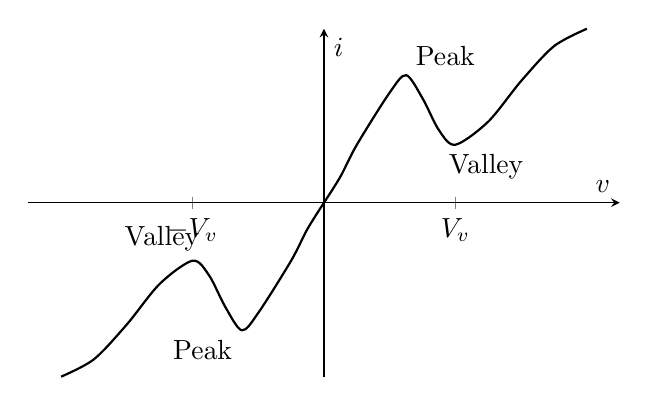
\begin{tikzpicture}
\begin{axis}[
    width=0.75\linewidth, height=6cm,
    axis lines=middle,
    xlabel={$v$}, ylabel={$i$},
    xmin=-0.9, xmax=0.9, ymin=-3, ymax=3,
    xtick={-0.4,0,0.4}, xticklabels={$-V_v$,$0$,$V_v$},
    ytick=\empty,
    domain=-0.8:0.8, samples=200,
    enlargelimits=false, clip=false,
]
    % Right half (positive voltage diode)
    \addplot[thick, smooth, domain=0:0.8]
      coordinates {
        (0.00,0.00) (0.05,0.45) (0.10,1.00) (0.20,1.90)
        (0.25,2.20) (0.30,1.80) (0.35,1.25) (0.40,1.00)
        (0.50,1.40) (0.60,2.10) (0.70,2.70) (0.80,3.00)
      };

    % Left half (mirror)
    \addplot[thick, smooth, domain=-0.8:0]
      coordinates {
        (-0.80,-3.00) (-0.70,-2.70) (-0.60,-2.10) (-0.50,-1.40)
        (-0.40,-1.00) (-0.35,-1.25) (-0.30,-1.80) (-0.25,-2.20)
        (-0.20,-1.90) (-0.10,-1.00) (-0.05,-0.45) (0.00,0.00)
      };

    % Labels
    \node[anchor=south west] at (axis cs:0.25,2.2) {Peak};
    \node[anchor=north west] at (axis cs:0.35,1.0) {Valley};
    \node[anchor=north east] at (axis cs:-0.25,-2.2) {Peak};
    \node[anchor=south east] at (axis cs:-0.35,-1.0) {Valley};
\end{axis}
\end{tikzpicture}
\caption{Symmetric \(i\!-\!v\) characteristic \(i = h(v)\) resulting from the circuit. Each half corresponds to one tunnel diode.}
\end{figure}

\subsection*{4. Explanation}
\begin{itemize}
  \item The \textbf{right-hand branch} (\(v>0\)) arises from the left diode’s forward characteristic.  
  \item The \textbf{left-hand branch} (\(v<0\)) arises from the right diode’s mirrored characteristic.  
  \item Around \(v=0\), both diodes are reverse-biased, producing nearly zero current.  
\end{itemize}

Thus, the overall element behaves as a \textbf{symmetric nonlinear resistor} 
with regions of \textbf{negative differential resistance}, as shown in the \(i=h(v)\) plot.
\section*{Single Tunnel-Diode Circuit and its \(i\text{--}v\) Characteristic}

The circuit shown below consists of a \textbf{tunnel diode} connected in series with a 
\SI{0.3}{V} bias source. The external terminals are labeled by voltage \(v\) and current \(i\).

\begin{figure}[htbp]
\centering
\begin{circuitikz}[american voltages]
  \fill[yellow!45] (-0.5,-0.5) rectangle (3.5,2.5);

  % Coordinates
  \coordinate (LT) at (0,2);
  \coordinate (LB) at (0,0);
  \coordinate (RT) at (3,2);
  \coordinate (RB) at (3,0);

  % Wires
  \draw (LT) to[short, o-] (RT);
  \draw (LB) to[short, o-] (RB);

  % Current arrow
  \draw[->] (0.4,2.25) -- ++(0.9,0) node[above] {$i$};

  % Vertical branch
  \coordinate (X) at (1.5,2);
  \draw (X) to[diode,l_=Tunnel diode] (1.5,1)
        to[battery1,l_=0.3\,V] (1.5,0);

  % Voltage polarity
  \node[left] at (LT) {$+$};
  \node[left] at (LB) {$-$};
  \node[left] at ($(LT)!0.5!(LB)$) {$v$};
\end{circuitikz}
\caption{Single tunnel-diode circuit with a \SI{0.3}{V} series bias source.}
\end{figure}

\subsection*{1. Voltage relationship}

Let \(v_d\) denote the voltage across the tunnel diode itself.  
Because the \SI{0.3}{V} battery is in series, the external voltage \(v\) is
\[
v = v_d + 0.3,
\quad \text{or equivalently} \quad
v_d = v - 0.3.
\]
Thus, the external current--voltage relationship becomes
\[
i = f(v - 0.3),
\]
where \(f(v_d)\) is the intrinsic diode characteristic.

---

\subsection*{2. Effect on the \(i\!-\!v\) curve}

The series \SI{0.3}{V} bias source shifts the entire tunnel-diode characteristic 
\textbf{leftward by 0.3 V} on the voltage axis.

\begin{itemize}
  \item When \(v < 0\): the diode is reverse biased (\(v_d < -0.3~\text{V}\)), and \(i \approx 0\).
  \item Around \(v \approx -0.3~\text{V}\): the diode just begins to conduct (tunneling region).
  \item For larger \(v\): the diode enters its negative-resistance region and then normal forward conduction.
\end{itemize}

---

\begin{figure}[htbp]
\centering
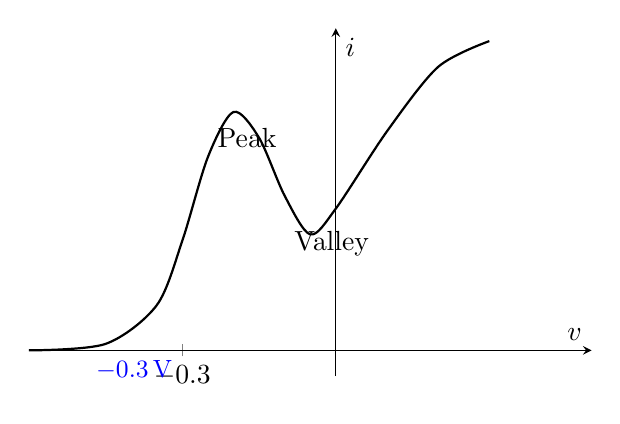
\begin{tikzpicture}
\begin{axis}[
    width=0.72\linewidth, height=6cm,
    axis lines=middle,
    xlabel={$v$}, ylabel={$i$},
    xmin=-0.6, xmax=0.5, ymin=-0.2, ymax=2.5,
    xtick={-0.3,0}, xticklabels={$-0.3$,$0$},
    ytick=\empty,
    enlargelimits=false, clip=false,
]
    % Shifted tunnel diode I–V
    \addplot[thick, smooth]
      coordinates {
        (-0.6,0.00) (-0.45,0.05) (-0.35,0.35)
        (-0.30,0.85) (-0.25,1.50) (-0.20,1.85)
        (-0.15,1.65) (-0.10,1.20) (-0.05,0.90)
        (0.00,1.10) (0.10,1.70) (0.20,2.20) (0.30,2.40)
      };

    % Label for shift
    \node[blue, anchor=north east] at (axis cs:-0.3,0) {\small $-0.3\,\mathrm{V}$};
    \node[anchor=south west] at (axis cs:-0.25,1.5) {Peak};
    \node[anchor=north west] at (axis cs:-0.10,1.0) {Valley};
\end{axis}
\end{tikzpicture}
\caption{\(i\!-\!v\) characteristic of the single tunnel-diode circuit.
The \SI{0.3}{V} source shifts the curve left by \SI{0.3}{V}.}
\end{figure}

\subsection*{3. Interpretation}

The \SI{0.3}{V} bias source provides a \textbf{DC offset} that moves the conduction
region of the tunnel diode away from the origin.  
From the external terminals:
\begin{itemize}
  \item For \(0 \le v < 0.29~\text{V}\), the current is nearly zero.
  \item When \(v \approx 0.3~\text{V}\), tunneling conduction begins.
  \item The external peak appears near \(v = -0.3~\text{V}\), showing the leftward shift caused by the bias source.
\end{itemize}

\[
\boxed{\text{The 0.3 V bias source shifts the tunnel diode's $i$--$v$ curve leftward by 0.3 V.}}
\]

\section*{為什麼在 \texorpdfstring{$v < 0.3\,\mathrm{V}$}{v < 0.3 V} 時出現負電流?}



考慮下圖的電路:一個 \textbf{隧道二極體(tunnel diode)} 串聯一個
\SI{0.3}{V} 的偏壓電池。  
外部端點的電壓為 \(v\),電流為 \(i\)。

\begin{figure}[htbp]
\centering
\begin{circuitikz}[american voltages]
  \fill[yellow!45] (-0.5,-0.5) rectangle (3.5,2.5);

  % 座標
  \coordinate (LT) at (0,2);
  \coordinate (LB) at (0,0);
  \coordinate (RT) at (3,2);
  \coordinate (RB) at (3,0);

  % 導線
  \draw (LT) to[short, o-] (RT);
  \draw (LB) to[short, o-] (RB);

  % 電流箭頭
  \draw[->] (0.4,2.25) -- ++(0.9,0) node[above] {$i$};

  % 垂直支路
  \coordinate (X) at (1.5,2);
  \draw (X) to[diode,l_=隧道二極體] (1.5,1)
        to[battery1,l_=0.3\,V] (1.5,0);

  % 電壓極性
  \node[left] at (LT) {$+$};
  \node[left] at (LB) {$-$};
  \node[left] at ($(LT)!0.5!(LB)$) {$v$};
\end{circuitikz}
\caption{含 0.3V 偏壓的隧道二極體電路。}
\end{figure}

---

\subsection*{1. 電壓關係}

設隧道二極體兩端的實際電壓為 \(v_d\)。  
由於串聯一個 \SI{0.3}{V} 的電池,有:
\[
v = v_d + 0.3 \quad \Rightarrow \quad v_d = v - 0.3.
\]
因此,當 \( v < 0.3\,\mathrm{V} \) 時,二極體端電壓 \( v_d < 0 \)。

即二極體處於\textbf{反向偏壓(reverse bias)} 狀態。

---

\subsection*{2. 隧穿效應與反向電流}

隧道二極體的耗盡層極薄(數奈米),
因此即使在反向偏壓下,
電子仍能利用 \textbf{量子隧穿效應(quantum tunneling)}
穿越能障。

這種反向穿隧電流方向與定義的正電流相反,
因此在外部量測上呈現為\textbf{負電流}:

\[
i < 0 \quad \text{(在 $v < 0.3\,\mathrm{V}$ 時)}.
\]

當 \(v > 0.3\,\mathrm{V}\) 時,二極體轉為正向偏壓,
開始產生正向隧穿電流,電流變為正值並迅速上升。

---

\subsection*{3. 外部 $i$--$v$ 特性}

\begin{figure}[htbp]
\centering
\begin{tikzpicture}
\begin{axis}[
    width=0.72\linewidth, height=6cm,
    axis lines=middle,
    xlabel={$v$}, ylabel={$i$},
    xmin=-0.1, xmax=0.5, ymin=-0.5, ymax=2.5,
    xtick={0,0.3}, xticklabels={$0$,$0.3$},
    ytick=\empty,
    enlargelimits=false, clip=false,
]
    % 負電流區
    \addplot[thick, smooth]
      coordinates {
        (0.00,-0.30) (0.10,-0.25) (0.20,-0.15)
        (0.25,-0.05) (0.30,0.00) (0.35,0.50)
        (0.40,1.10) (0.45,1.80)
      };

    % 標註
    \node[blue, anchor=south west] at (axis cs:0.3,0) {\small \text{0.3 V}};


    \node[anchor=north east, text width=3.8cm, align=right] at (axis cs:0.18,-0.2)
      {\small 反向隧穿電流(負電流)};
\end{axis}
\end{tikzpicture}
\caption{在 $v<0.3\,\mathrm{V}$ 時的反向隧穿電流導致 $i<0$。}
\end{figure}

---

\subsection*{4. 物理解釋(能帶觀點)}

\begin{itemize}
  \item 當 $v < 0.3\,\mathrm{V}$ 時,二極體內部電壓 $v_d < 0$,
        其 $n$ 區填滿的能態與 $p$ 區空能態對齊,
        電子可穿隧從 $p$ 區至 $n$ 區,
        電流方向與外部定義的正電流相反,故 $i < 0$。
  \item 當 $v \approx 0.3\,\mathrm{V}$ 時,
        反向偏壓被抵消,隧穿電流趨近於零。
  \item 當 $v > 0.3\,\mathrm{V}$ 時,
        二極體正向偏壓,電子由 $n$ 區注入 $p$ 區,
        出現正向隧穿電流,$i > 0$。
\end{itemize}

---

\subsection*{5. 總結}

\begin{tcolorbox}[colback=yellow!5!white, colframe=black!75, boxrule=0.8pt, title=結論]
在 \( v < 0.3\,\mathrm{V} \) 時,
由於隧道二極體受到反向偏壓,
產生方向相反的反向隧穿電流,
因此量測到的外部電流為負值。
\end{tcolorbox}

\section*{參考資料}
\[
M = [v_1, v_2],
\qquad
\overline{M^{-1}} = (M^{-1})^{*}.
\]
\[
M = [v_1, v_2],
\qquad
\overline{M^{-1}}.
\]
\section*{推導}
\[
\dot{z}_1 = \lambda_1 z_1, 
\qquad 
\dot{z}_2 = \lambda_2 z_2.
\]

其解為
\[
z_1(t) = z_{10} e^{\lambda_1 t}, 
\qquad 
z_2(t) = z_{20} e^{\lambda_2 t}.
\]

消去時間變數 \(t\),由第一式得
\[
t = \frac{1}{\lambda_1} \ln \frac{z_1}{z_{10}}.
\]

代入第二式得
\[
z_2 = z_{20} e^{\lambda_2 \left( \frac{1}{\lambda_1} \ln \frac{z_1}{z_{10}} \right)}
     = z_{20} \left( \frac{z_1}{z_{10}} \right)^{\lambda_2 / \lambda_1}
     = c\, z_1^{\lambda_2 / \lambda_1},
\]
其中
\[
c = z_{20} z_{10}^{-\lambda_2 / \lambda_1}.
\]
\end{document}
